\subsection{Level1.1: OR問題が解けることの確認}
\subsubsection{学習が収束する回数}
指定されたシード値を用いた際の、学習が終了した回数を表
\ref{table:level1.1}に示す。

\begin{table}[htb]
 \begin{center}
  \caption{OR問題の学習に要した回数}
  \label{table:level1.1}
  \begin{tabular}[htb]{r|l} \hline
   シード値 & 収束した回数 \\ \hline \hline
   1000 & 97 \\ \hline
   2000 & 91 \\ \hline
   3000 & 112 \\ \hline
   4000 & 109 \\ \hline
   5000 & 94 \\ \hline
   6000 & 100 \\ \hline
   7000 & 101 \\ \hline
   8000 & 115 \\ \hline
   9000 & 114 \\ \hline
   10000 & 95 \\ \hline
  \end{tabular}
 \end{center}
\end{table}

また、横軸を学習回数、縦軸を誤差としたときの学習結果を
\ref{graph:level1.1-1}と\ref{graph:level1.1-2}に示す。

\begin{figure}[h]
 \begin{center}
  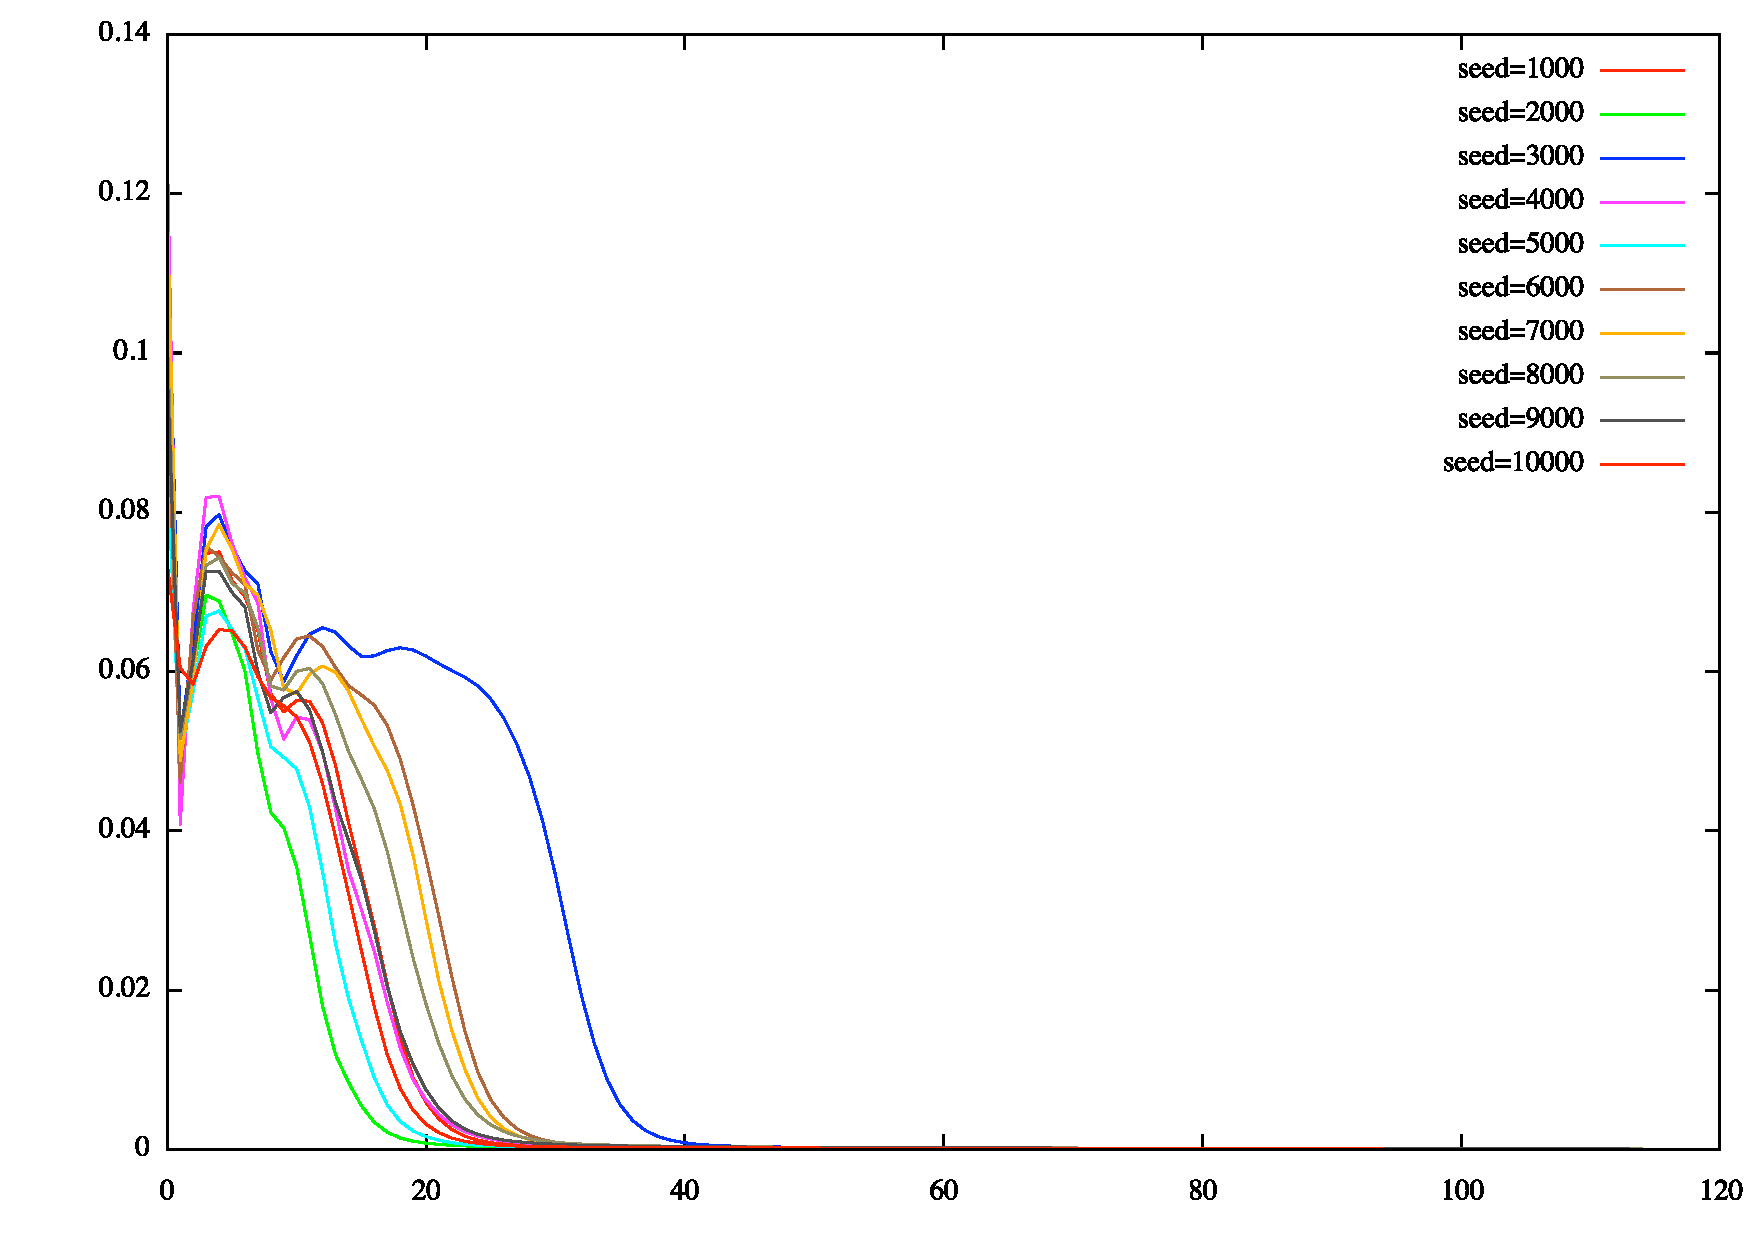
\includegraphics[width=10.0cm]{figs/ex.pdf}
  \caption{シード値を変更して得られた10回分の学習結果}
  \label{graph:level1.1-1}
 \end{center}
\end{figure}

\begin{figure}[h]
 \begin{center}
  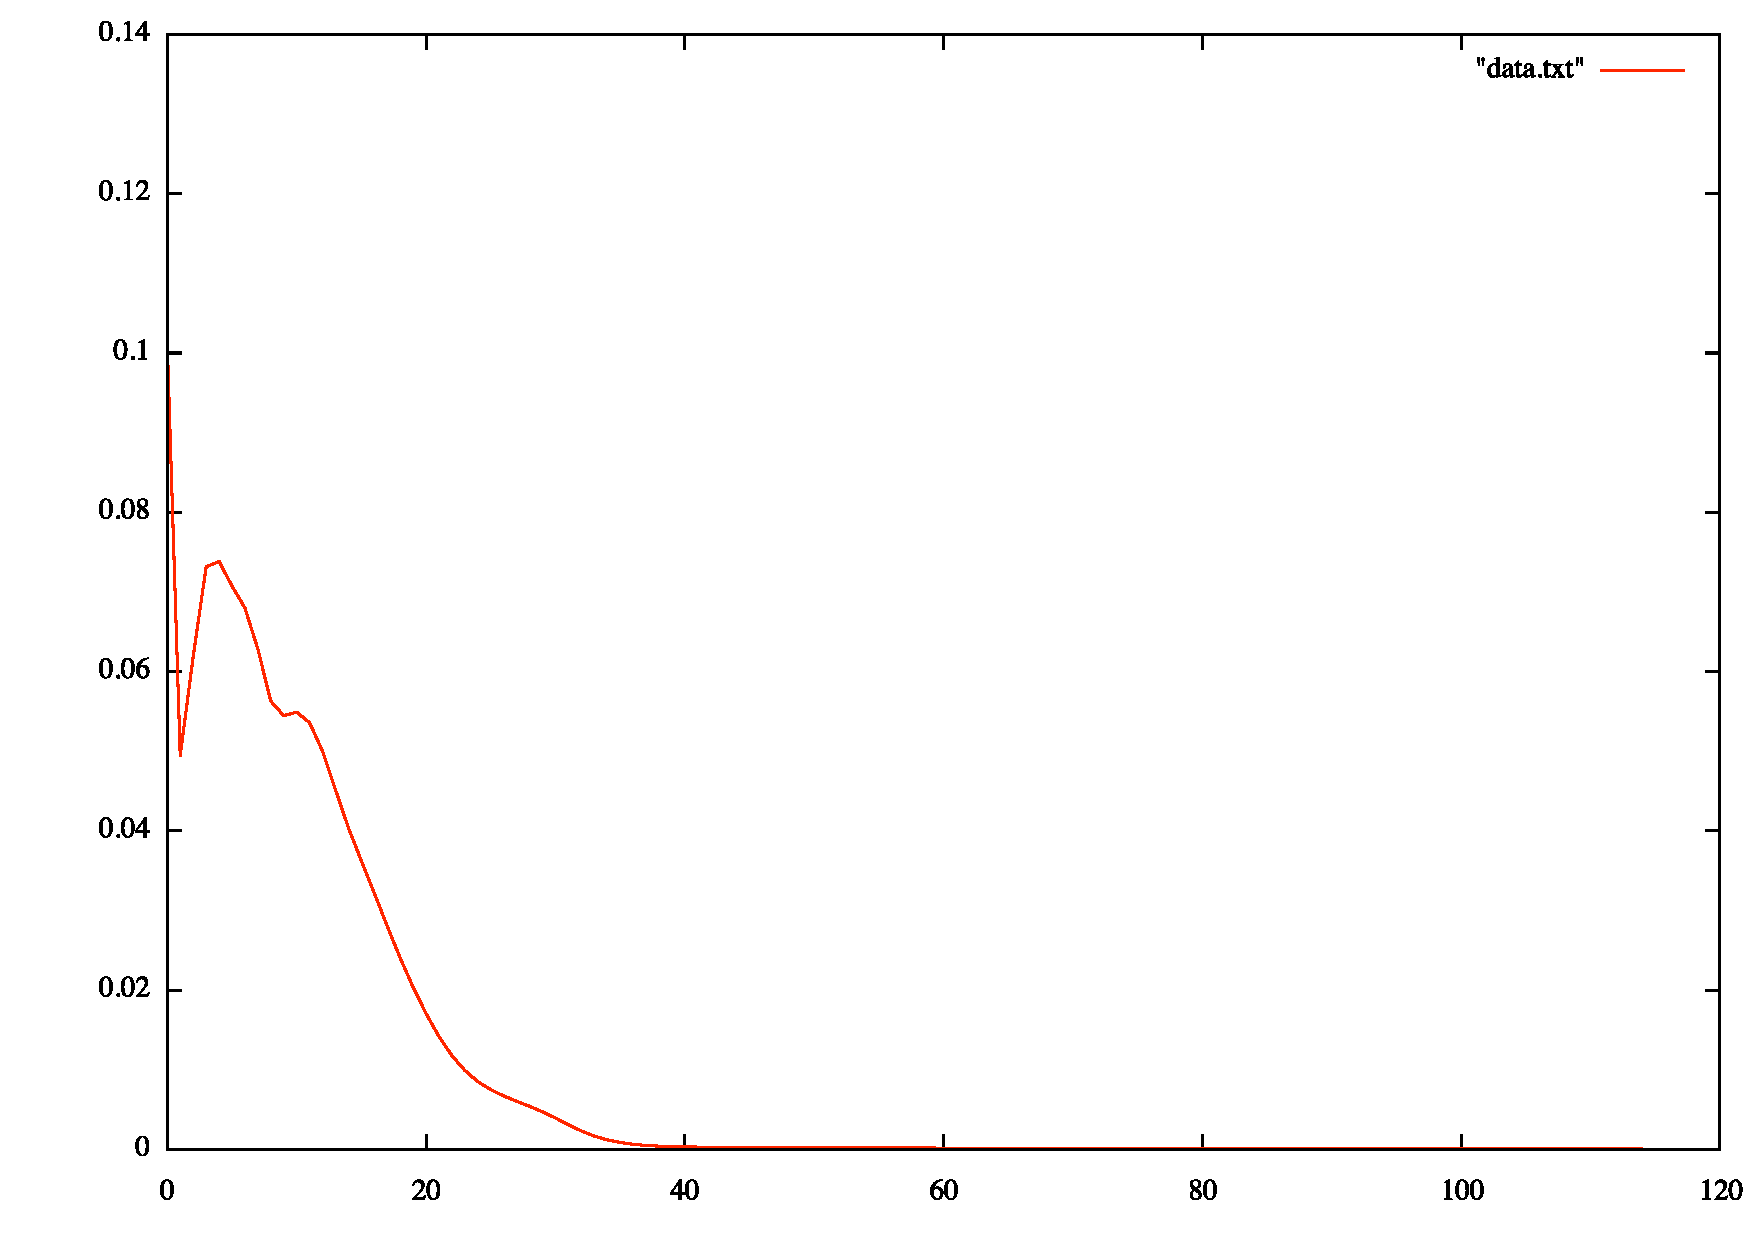
\includegraphics[width=10.0cm]{figs/ex_ave.pdf}
  \caption{10回分の学習結果を平均した結果}
  \label{graph:level1.1-2}
 \end{center}
\end{figure}

\subsubsection{考察}
\ref{table:level1.1}より、シード値が変わっても、収束するまでの学習回数はおおよそ100回ぐらいになる。

